\documentclass[11pt]{article}

\usepackage{graphicx}
%\usepackage{amsmath}

\usepackage{tcolorbox}
\usepackage[english]{babel}
\usepackage[square,numbers]{natbib}
\bibliographystyle{abbrvnat}

\usepackage{hyperref}
\hypersetup{colorlinks,
citecolor=blue
}
\hypersetup{
    % citecolor=blue
    colorlinks=true,
    linkcolor=magenta,
    filecolor=magenta,      
    urlcolor=cyan
 %   pdfpagemode=FullScreen,
    }
%---------------------
%\input{packages}


\usepackage{amsmath}            % extensions for typesetting of math
%\usepackage{amsfonts}          % math fonts
%\usepackage{amssymb}
%\usepackage{amsthm}            % theorems, definitions, etc.
%\usepackage{bbding}            % various symbols (squares, asterisks, scissors, ...)
\usepackage{bm}                 % boldface symbols
\usepackage{cases}              % equation cases
\usepackage{tensor}
\usepackage{algorithm}
\usepackage{algpseudocode}
\usepackage{algorithmicx}
\usepackage{listings}           % adding inlinecode

\newcommand{\inlinecode}[1]{\colorbox{lightgray}{\lstinline[breaklines=true,basicstyle=\ttfamily]{#1}}}

\newcommand{\fgrad}{\tensorq{F}}
%\renewcommand{\identity}{\tensorq{I}}
\newcommand{\density}{\rho}
\newcommand{\generictensorc}{\mathrm{A}}
\newcommand{\Div}{\operatorname{Div}}
\newcommand{\pkstress}{\tensorq{T}_{\mathrm{R}}}
\newcommand{\Cof}{\operatorname{Cof}}
\newcommand{\D}[1]{\mathrm{d#1}}
% \usepackage[colorlinks,allcolors=cyan!70!black]{hyperref}

% Uncomment if using biblatex
% \addbibresource{sample.bib}

\usepackage{xcolor, color, soul}
\sethlcolor{green}

\usepackage{lipsum}
%-----------------------------------------------------
% \definecolor{lightcream}{rgb}{0.97, 0.97, 0.86}  % defining a lighter cream color
\usepackage{xcolor}  % to define colors
\usepackage{mdframed}  % for framing

\definecolor{lightgray}{gray}{0.9}  % defining light gray color




\title{OrganL User Manual}
\author{Christoph Allolio, Hina Arif and Jovi K}

\date{Version 1.0 - 26.4.2024}

\begin{document}

\maketitle
\begin{center}
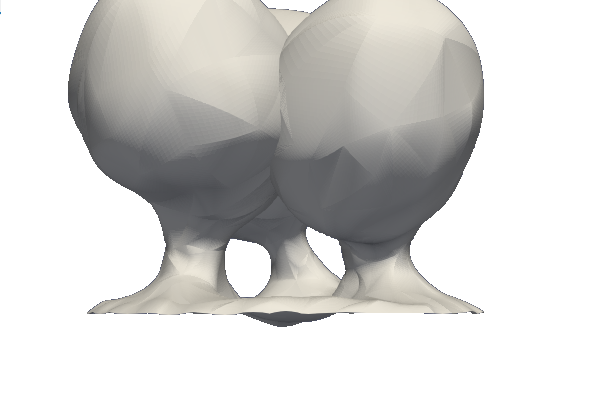
\includegraphics[width=0.5\linewidth]{buddings.png} \\

\includegraphics[width=0.5\linewidth]{logo.png}

\end{center}
 \pagenumbering{gobble}
\newpage
\pagenumbering{arabic}
\section{Introduction and Disclaimer}

% nagata and nag\_mix are simulation codes used to study the evolution of mitochondrial cristae. They account for all mechanical and elastic properties of the system. The standard nagata simulation ignores lipid composition, while nag\_mix moves lipids in a neutral manner and maintains the balance of both leaflets. The codes are designed to finesse the file into mitochondrial cristae; hence it's necessary to set the volume rather than the pressure.

\textbf{OrganL} is a Monte Carlo simulation tool for evolving (sub)cellular scale membrane structures. The program implements a variety of curvature-elastic energy functionals and couplings. It is designed to be extensible with the final goal of simulating entire cellular organelles. The program is written in portable C++ and designed for parallel execution. This manual is provided together with a distribution of the program including several examples. The method and the tool are published in the Biophysical Journal \url{https://doi.org/10.1016/j.bpj.2024.04.028}. Cite this paper when using OrganL\\
\vspace{0.5 cm}

\noindent
\small{
WHEN THE PROGRAM IS LICENSED FREE OF CHARGE, THERE IS NO WARRANTY
FOR THE PROGRAM, TO THE EXTENT PERMITTED BY APPLICABLE LAW.  EXCEPT WHEN
OTHERWISE STATED IN WRITING THE COPYRIGHT HOLDERS AND/OR OTHER PARTIES
PROVIDE THE PROGRAM "AS IS" WITHOUT WARRANTY OF ANY KIND, EITHER EXPRESSED
OR IMPLIED, INCLUDING, BUT NOT LIMITED TO, THE IMPLIED WARRANTIES OF
MERCHANTABILITY AND FITNESS FOR A PARTICULAR PURPOSE.  THE ENTIRE RISK AS
TO THE QUALITY AND PERFORMANCE OF THE PROGRAM IS WITH YOU.  SHOULD THE
PROGRAM PROVE DEFECTIVE, YOU ASSUME THE COST OF ALL NECESSARY SERVICING,
REPAIR OR CORRECTION.
IN NO EVENT UNLESS REQUIRED BY APPLICABLE LAW OR AGREED TO IN WRITING
WILL ANY COPYRIGHT HOLDER, OR ANY OTHER PARTY WHO MAY MODIFY AND/OR
REDISTRIBUTE THE PROGRAM, BE LIABLE TO YOU FOR DAMAGES,
INCLUDING ANY GENERAL, SPECIAL, INCIDENTAL OR CONSEQUENTIAL DAMAGES ARISING
OUT OF THE USE OR INABILITY TO USE THE PROGRAM (INCLUDING BUT NOT LIMITED
TO LOSS OF DATA OR DATA BEING RENDERED INACCURATE OR LOSSES SUSTAINED BY
YOU OR THIRD PARTIES OR A FAILURE OF THE PROGRAM TO OPERATE WITH ANY OTHER
PROGRAMS), EVEN IF SUCH HOLDER OR OTHER PARTY HAS BEEN ADVISED OF THE
POSSIBILITY OF SUCH DAMAGES.}


\begin{tcolorbox}[colback=red!5!white,colframe=red!75!black,title=Warning]
This is not free software (c) 2020-2024 Christoph Allolio \\
The code is subject to the Academic Software Licence (see LICENSE file for details)
\end{tcolorbox}
% \begin{enumerate}
%     \item \textbf{Comprehensive Mechanical and Elastic Properties:} \textbf{OrganL} accounts for all relevant mechanical and elastic properties of the system, ensuring accurate and reliable results in modeling and analysis.

%     \item \textbf{Lipid Composition Handling:} The \textbf{OrganL} simulation primarily focuses on the mechanical aspects without taking lipid composition into consideration. However, it also incorporates lipid composition and simulates lipid movement. Importantly, it maintains a balanced distribution across both leaflets of the membrane, reflecting more complex biological realities.
    
%     \item \textbf{Advanced Interpolation Scheme:} The tools incorporate a powerful yet intuitive interpolation scheme, overcoming previous limitations observed with the Nagata interpolant.

%     \item \textbf{Mitochondrial Cristae Fine-tuning:} This code enables the users to finesse simulations to accurately replicate the intricate structures and evolution of mitochondrial cristae. Rather than working with pressure, which might be more common in generic simulations, users set the volume to achieve high precision in modeling the unique environment of the cristae.

%     \item \textbf{Validation against Helfrich Hamiltonian:} The simulations have been validated against the behavior of the known rotationally symmetric solutions of the Helfrich Hamiltonian, reinforcing their reliability and efficacy.

%     \item \textbf{Capability for Advanced Methods:} Beyond the basic Helfrich minima, the robust surface description offered by the tools allows for the inclusion of lipid moves, further enhancing the detail and depth of simulations.

%     \item \textbf{Extensibility:} The underlying architecture of the software is designed for potential enhancements and additions. This means that future versions could incorporate even more complex phenomena, such as explicit protein interactions, cytoskeleton inclusion, mitochondrial morphology and more.
% \end{enumerate}

% These features combine to offer a holistic and versatile toolset for researchers and experts focused on the study of biomembranes, mitochondrial morphology involving fission, fusion and cristae formation and the broader intricacies of lipid membranes.

% These features come together to provide a comprehensive and flexible toolset for researchers and experts who are dedicated to studying biomembranes, including mitochondrial morphology encompassing processes like fission, fusion, and cristae formation, as well as the broader complexities of lipid membranes.

\newpage

\tableofcontents

\newpage

\section{Installation and System Requirements}

OrganL is written in C++ and can be compiled without the use of nonstandard external libraries. During development, it has been compiled with GNU C++ 11.4.0\cite{gcc}, with the default standard. This should correspond to C++ 17. 
To compile the software, the CMake build system Version 3.0\cite{cmake} or higher is recommended.
Parallel execution requires linking to the OpenMP libary\cite{openmp}. 
Static Linux binaries are available for x86-64 processors. 
Rudimentary Python bindings are available and can be included by editing the CMakeList.txt file. These bindings require PyBind11\cite{pybind11}. Users are encouraged to report the result of compiling organl for Windows or ARM, Android and whatever
is required. It is also possible to create rudimentary python bindings uncommenting lines in the CMakeLists.txt file. These bindings are not documented.

\subsection{Linux Environment}
On a normal Ubuntu machine, building the software from the source directory should be as easy as

\begin{mdframed}[backgroundcolor=lightgray, linecolor=lightgray]
\begin{verbatim}
cd build
cmake ..
make
\end{verbatim}
\end{mdframed}

The resulting executable, is called organl. It is dynamically linked. To create a static executable use 
\begin{mdframed}[backgroundcolor=lightgray, linecolor=lightgray]
\begin{verbatim}
cmake .. -DSTATIC_LINK
\end{verbatim}
\end{mdframed}
This executable should be portable by default, but may not compile if you use an exotic distribution. It does not require any further installation. In our cluster it executes on wide variety of Linux versions without setting special paths.

If cmake is not available or fails, it is possible to build a parallel optimized version in one line using GCC:
\begin{mdframed}[backgroundcolor=lightgray, linecolor=lightgray]
\begin{verbatim}
g++ main.cpp -fopenmp -o organl -O3
\end{verbatim}
\end{mdframed}
This has to be executed in the source code directory.

\subsection{Building on Microsoft Windows}
Start by setting up GCC and the MinGW libraries on Windows. It is recommended to use the standalone build from \href{https://winlibs.com/}{WinLibs} since it includes compilers and build tools (cmake and compilers like g++. clang++, clang-cl, etc.) and MinGW. Don't forget to add \inlinecode{mingw32\\bin} or \inlinecode{mingw64\\bin} to the environment variable \inlinecode{PATH}.
Further run the following commands in Command Prompt or Powershell from the source directory:
\begin{mdframed}[backgroundcolor=lightgray, linecolor=lightgray]
\begin{verbatim}
mkdir build
cd build
cmake .. -G "MinGW Makefiles" -DCMAKE_CXX_COMPILER=g++
mingw32-make
\end{verbatim}
\end{mdframed}
The expected outcome is generating three executables named \inlinecode{organl.exe}, \inlinecode{helf-} \inlinecode{ins.exe} and \inlinecode{angle.exe}. 

Note that using other compilers like clang++ will require either explicitly specifying libraries or installing other dependencies, for example using llvm-clang based compiler would require you to have MSVCRT (Microsoft Visual C++ Runtime) on your system since it's incompatible with the GCC library. Also you will need to change the cmake script appropriately. \\

Generating static binaries might require specifying the full path of certain MinGW libraries in the \inlinecode{CMakeLists.txt}, for example like so,
\begin{mdframed}[backgroundcolor=lightgray, linecolor=lightgray]
\begin{verbatim}
target_link_libraries(organl "D:/mingw64/bin/libdl.dll")
\end{verbatim}
\end{mdframed}
If cmake fails for some reason, it is possible to build a parallel optimized version in one line using GCC:
\begin{mdframed}[backgroundcolor=lightgray, linecolor=lightgray]
\begin{verbatim}
g++ ../main.cpp -fopenmp -o organl.exe -O3
\end{verbatim}
\end{mdframed}

The build instructions in this subsection has been verified using GNU 13.2.0 and OpenMP 5.0.

\subsection{Cross-compiling on Linux for MacOS}
This section aims to explain the setup for cross-compiling with Linux for MacOS in clang using the OSXCross\cite{osxcross} toolchain. For detailed instruction, refer the OSXCross project official \href{https://github.com/tpoechtrager/osxcross?tab=readme-ov-file#how-does-it-work}{Github page}. The build instructions are  - 
Download and build OSXCross toolchain using \inlinecode{clang} and install in \inlinecode{<path>/osxcross} by running:
\begin{mdframed}[backgroundcolor=lightgray, linecolor=lightgray]
\begin{verbatim}
TARGET_DIR=<path> ./build.sh
\end{verbatim}
\end{mdframed}
Now add \inlinecode{<path>/target/bin} to the PATH variable to invoke the cross-compiler in terminal. This is essential everything that follows.
Compiling for MacOS requires its SDK and other compactible libraries. The SDK may be extracted from the official Xcode Disk image. Start by downloading Xcode from \href{https://developer.apple.com/download/all/}{Apple's Website}, you might be required to sign in with an Apple ID. Install dependencies \inlinecode{make}, \inlinecode{libssl-devel}, \inlinecode{lzma-devel} and \inlinecode{libxml2-devel}. Now run, 
\begin{mdframed}[backgroundcolor=lightgray, linecolor=lightgray]
\begin{verbatim}
./tools/gen_sdk_package_pbzx.sh <xcode>.xip
\end{verbatim}
\end{mdframed}
Move the compiled SDK into \inlinecode{tarballs/} directory. Compile the inlinecode{ osxcross-macports} in the osxcross directory by running the corresponding cmake file. These contain headers and openmp compactibility among others. Now the toolchain is ready to use. It may be invoked just like gcc or clang, but by compiler binary with \inlinecode{o64-clang} instead. To cross-compile organl now, navigate to the \inlinecode{source/} directory and run the following:
\begin{mdframed}[backgroundcolor=lightgray, linecolor=lightgray]
\begin{verbatim}
o64-clang++ -fopenmp -v ../main.cpp -o organl_macos
\end{verbatim}
\end{mdframed}
Similarly compile other required binaries like \inlinecode{angle_macos} or \inlinecode{helfins_macos} by replacing \inlinecode{main.cpp} with \inlinecode{angle.cpp} or \inlinecode{helfins.cpp} respectively. Compiling the source using cmake and OSXCross toolchain is possible but requires quite extended configurations, and requires the paths to various libraries to be specified manually since the cmake doesn't have any generator for this toolchain. Compiling fully static binaries for MacOS is not possible using the flag \inlinecode{-static} for reasons given \href{https://stackoverflow.com/questions/3801011/ld-library-not-found-for-lcrt0-o-on-osx-10-6-with-gcc-clang-static-flag}{here}. \\\\
Some commonly encountered problems are listed below:
\begin{itemize}
    \item fatal error: 'omp.h' file not found: Easiest way to solve this is to copy paste \inlinecode{omp.h} file from gcc to \inlinecode{/usr/local/lib/clang/17/include}. The actual paths might vary depending on installation but should be similar.
    \item osxcross-macport public key not matching: Make sure you downloaded the original files from Offical apple's website. If the problem persists commend out \inlinecode{exit 1} in the \inlinecode{osxcross-macport} code.
    \item ld: library not found for -lomp; clang++: error: linker command failed - This is due to missing libomp.dylib in the PATH - install libomp using osxcross-macports  to \inlinecode{/usr/local/lib} or add the path if already installed.
\end{itemize}
Strictly speaking, since these problems are not directly related to our package, its best to refer OSXCross \href{https://github.com/tpoechtrager/osxcross/issues}{Issues page} for these and other problems that might arise.\\

The instructions in this subsection is tested using Xcode Disk image version 15.2 and targets MacOS Sonoma v14 and Darwin v23 systems. The MacOS binaries in the \inlinecode{binaries/} directory are NOT runtime validated.

\section{Usage}

Copy the appropriate \textbf{organl} binary for your platform from \inlinecode{/binaries/} into this folder. Under UNIX, in its own directory, the program can be executed using the command line:
\begin{mdframed}[backgroundcolor=lightgray, linecolor=lightgray]  % setting the frame and background color to lighter cream
\begin{verbatim}
./organl {filename.obj} [ADE | CHF | EAP | EAH | DCH | DCG ] 
  [ LIP ] [ BNE | TAU ]
\end{verbatim}

% \begin{verbatim}
% ./nag_mix {filename.obj} [ADE | CHF | EAP | DCH ] [ LIP ]
% \end{verbatim}
% \end{mdframed}
% For nagata, use:
% \begin{mdframed}[backgroundcolor=lightgray, linecolor=lightgray]  % setting the frame and background color to lighter cream

% \begin{verbatim}
% ./nagata {filename.obj} [ADE | CHF | EAP | DCH ] [ LIP ]
% \end{verbatim}
\end{mdframed}
Here, arguments in curly brackets are necessary, whereas arguments in square brackets are optional. The filename.obj is a mesh file in wavefront obj format. The first set of options in square brackets refers to the choice of energy functional and the [LIP] option in the command line is used to enable lipid mixing. The last two terms refer to separate edge energies.
If no energy functional is specified, the DCH option is used.
\section{Features}

The core functionality of the code is to perform Metropolis-Hastings Monte Carlo to sample the Boltzmann distribution of thin-shell energy functionals associated with the deformation of liquid biomembranes.

For a free membrane, the Helfrich free energy $F_{HF}$ can be expressed as:
% , supplemented by surface tension ($\sigma$) and pressure ($p$) terms can be expressed as:

 \begin{equation}
  F_{HF} = \int_{Surf.} \D{A}  \bigg\{ \frac{{\kappa}}{2} (H-J_S)^2 \bigg\}.
  % F = \int_{Surf.} \D{A}  \bigg\{ \frac{{\kappa}}{2} (H-J_S)^2 + \bar{\kappa} K_G  + \sigma \bigg\} +\int_{Vol} \D{V} p.
  \label{eq:helf}
 \end{equation}
 
In this equation, the geometric quantities include mean curvature ($H$), and the area element ($\mathrm{d}A$). The material parameters consist of bending rigidity ($\kappa$), and spontaneous or intrinsic curvature ($J_S$). 
\begin{tcolorbox}[colback=orange!5!white,colframe=orange!75!black,title=Clarification]
\begin{itemize}
    \item The pure Helfrich functional without $J_s$ is scale invariant, and requires additional input for simulations. 
    \item In agreement with biological convention, the curvature $H$ is defined as $c_1 + c_2$, with $c_n$ the principal curvatures of the surface. The curvature of a surface depends on the orientation of normals chosen by the user. 
    \item $J_s$, also sometimes written as $c_0$ is defined in relation to $H$.
\end{itemize}
\end{tcolorbox}
\subsection{Units}
The program uses $kT$ units. While there is no direct reference to any length scale, we recommend \textrm{nm} as a unit, and recommend to use it when providing lipid specific information. 

\subsection{Implemented Energy Functionals}
As indicated by the command line options, various energy functionals are available, allowing users to choose the most suitable energy functional for their simulation requirements. Here's a brief overview of the available parameters:
\\
%-------------------------------------------------------
% %are
% %\begin{equation}
% % \Phi =  \int_0^1 d\eta \int_0^\eta d\zeta f(\eta,\zeta) \| \vec{x}_\eta(\eta,\zeta) \times \vec{x}_\zeta(\eta,\zeta)\| 
% The surface integral is summed over all patches and in each patch is discretized on the domain of the interpolant using a seventh-order Gaussian quadrature scheme\cite{https://doi.org/10.1002/nme.1620120107}. Note the facility of, e.g. constructing parallel planes for accounting explicitly for separate monolayers and the availability of a reasonable direct way to evaluate Gaussian curvature. On the level of the code, different energy functionals are available via subclassing. Some are described in the Supporting Information, most notably an implementation of area difference elasticity (ADE)\cite{PhysRevA.44.1182} via control of the integrated mean curvature. Local curvatures can be expressed in a simplified manner by the coefficients. Details are given in the Supporting Information.
% L(H-J_S)^2
%-------------------------------------------------------------------
\noindent
\textbf{CHF (Constrained Helfrich Functional)}
The CHF represents the pure Helfrich functional with additional constraints implemented using penalities. (So strictly speaking they are restraints.) 
 It can be expressed as
 \begin{equation}
   F_{CHF} = F_{HF} +     \frac{\lambda_0}{2} \bigg(A_0- \int_{Surf.} \mathrm{d}A\bigg)^2  +  \frac{\lambda_1}{2} \bigg(V_0-\int_{Vol} \mathrm{d}V\bigg)^2,
  \end{equation}
 where $F_{HF}$ is the standard Helfrich energy.
This approach can also be reinterpreted as being "variationally equivalent" to the standard version of the Helfrich Energy with pressure $p$ and surface tension $\sigma$ 
\begin{equation}
 % F = int_{Surf.} \gamma dA,
  F = \int_{Surf.} dA  \bigg\{ \frac{{\kappa}}{2} (H-J_S)^2 + \sigma \bigg\}  + \int_{Vol} p \mathrm{d}V,
  % \int_{Surf.} \D{A} \sigma ,
\end{equation}
where $\sigma$ can be computed from a second order elastic modulus $K_A$
\begin{equation}
  \sigma  =  K_A(A-A_0).
\end{equation}
and $p$ is compute from an analogous compressibility property
\begin{equation}
  p  =  -K_B(V-V_0).
\end{equation}
This means that the penalties $\lambda_i$ can also be assigned physical meaning, given that no material is fully incompressible. In the energy file the Energy is reported split into $F_{HF}$ and $F_{C} = F_{CHF}-F_{HF} $, where $F_C$ is reported as \textit{Constraint Energy}. \\
\noindent
\begin{tcolorbox}[colback=orange!5!white,colframe=orange!75!black,title=Clarification]
\begin{itemize}
    \item The Volume $V$ is computed using the divergence theorem as stated in the manuscript. Please check the normal orientation of your mesh.  
    \item the values of $\lambda_i$ and V$_0$ and A$_0$ refer to global parameters and need to be set in the run control via LAMBDA and DEF keywords.
    \end{itemize}

\end{tcolorbox}

\noindent
\textbf{Requires}: 2 $\textbf{LAMBDAS}$ and 2 $\textbf{DEF}$ (A$_0$ and V$_0$) \\
\noindent \\
\vspace{0.2 cm}
\textbf{DCH (Double Constraint Helfrich): [DEFAULT]}
DCH adds an additional \textit{per face} restraint to yield 
\begin{equation}    
 F_{DCH} = F_{CHF} + \sum_i \frac{K_i}{2}(A_i-A_{0,i})^2 
 , 
 \end{equation}
 or fully 
 \begin{equation}
      \frac{\lambda_0}{2} \bigg(A_0- \int_{Surf.} \mathrm{d}A\bigg)^2  +  \frac{\lambda_1}{2} \bigg(V_0-\int_{Vol} \mathrm{d}V\bigg)^2 
+ \sum_i \frac{K_i}{2}(A_i-A_{0,i})^2 
  ,
  \end{equation}
where 
\begin{equation}
A_i = \int_{S_i} \mathrm{d}A 
\end{equation}
In this case, $K_i$ and $A_{0,i}$ are local and stored on the faces, and $A_i$ is computed for each face. These values can be set in the mesh properties, and can in principle be computed on the fly during the simulation. \\
This additional constraint can be used to tightly control mesh quality, where necessary, to control lipid population and even to restrict membrane fluidity. \textbf{Note},
\begin{itemize}
    \item the energy contributions due to $K_i$ are reported as part of the $Energy$ and not the constraint energy $F_C$.
    \item it is possible to set both $\lambda_i$ and $K_i$ to zero reducing the energy to CHF or EAH. 
\end{itemize}
\begin{tcolorbox}[colback=red!5!white,colframe=red!75!black,title=Warning]
\begin{itemize}
    \item The $K_i$ added to the faces will affect the penalty energy scale $I$ even when DCH is not used. 
    \item Setting $A_{0,i}$ in a way that is incompatiple with $A_0$ can lead to unpredictable behavior. It is recommended to set $A_0 = \sum_i A_{0,i}$
    \item High values of $K_i$ will lead to lower acceptance probabilities and steps.
    \end{itemize}
\end{tcolorbox}

\noindent
\textbf{Requires}: 2 $\textbf{LAMBDAS}$ and 2 $\textbf{DEF}$ (A$_0$ and V$_0$) \\
\noindent \\
\vspace{0.2 cm} \\
\textbf{EAH (Elastic Area Helfrich):}
This functional allows users to study the Helfrich functional without global restraints. It is equivalent to DCH with both $\lambda_i = 0$
\begin{equation}    
 F_{EAH} = F_{HF} + \sum_i \frac{K_i}{2}(A_i-A_{0,i})^2
 . 
 \end{equation}
\noindent
This should be the fastest running and simplest energy functional implemented. Unfortunately, the organl command line does not give access $F_{HF}$ directly. The energy can be evaluated from a restart using the tool \begin{verbatim}helfins \end{verbatim} \\
\noindent
\textbf{Requires}: 0 $\textbf{LAMBDAS}$ and 0 $\textbf{DEF}$ \\
\noindent \\
\vspace{0.2 cm} \\
\textbf{EAP (Elastic Area Pressure):}
The EAP functional can be used to simulate the effect of constant pressure. The extended functional can be expressed as:
 \begin{equation}
 F_{EAP} = F_{HF} - \int_{Vol} \D{V} p + \sum_i \frac{K_i}{2}(A_i-A_{0,i})^2 = F_{EAH} - \int_{Vol} \D{V} p.
 \end{equation}
Note, the constant pressure has to be supplied as a \textbf{DEF} and care has to be taken with the sign. At present, positive pressure increases $V$. There is no constraint energy. This can be a good choice for a subsystem.

\begin{tcolorbox}[colback=orange!5!white,colframe=orange!75!black,title=Clarification]
    What limits the volume in this simulation is the elastic energy of the faces, $K_i$ and $p$ must be chosen together, 
    e.g. by comparing tension and pressure for a certain stretch of the surface. 

\end{tcolorbox}

\noindent
\textbf{Requires}: 0 $\textbf{LAMBDAS}$ and 1 $\textbf{DEF}$ ($p$) \\
\noindent \\
\vspace{0.2 cm} \\
\noindent \\
\vspace{0.2 cm} \\
\textbf{DCG (Double Constraint Gaussian Curvature):}
The DCG functional can be used to simulate the effect of a locally different Gaussian bending modulus $\overline{\kappa}$ and the Gaussian curvature $K$. The extended functional can be expressed as
 \begin{equation}
 F_{DCG} = F_{DCH} + \int_{Surf.} \overline{\kappa}K  \mathrm{d}A.
 \end{equation}
The modulus $\overline{\kappa}$ is usually negative and very hard to measure, some reasonable first guess would be $-0.8 \kappa$.  The restraints are the same as those for the Double constraint Helfrich Energy.
\begin{tcolorbox}[colback=orange!5!white,colframe=orange!75!black,title=Clarification]
    Note, that this only makes sense if $\overline{\kappa}$ is highly inhomogeneous, as otherwise the Gauss-Bonnet theorem will turn the integral into a topological constant. If your system has an open boundary, you should choose a Bonnet edge energy term in addition to this functional. 
\end{tcolorbox}

\noindent
\textbf{Requires}: 2 $\textbf{LAMBDAS}$ and 2 $\textbf{DEF}$  \\
\noindent \\
\vspace{0.2 cm} \\
% Firstly, we note that $V$ can be obtained from the divergence theorem using the spatial coordinate $\mathbf{r}$ as \begin{equation}
%  V = \frac{1}{3} \int_{Vol} \nabla \cdot {\vec{r}} \D{V} =  \frac{1}{3} \int_{Surf.}   \vec{x} \cdot \hat{\vec{n}} \D{A},
% \end{equation}
% where $\hat{\vec{n}}$ is the surface unit normal vector as computed from the patch interpolant $\vec{x}$. Therefore, it is sufficient to work with surface integrals to evaluate all of $F$.

\noindent

\noindent
\textbf{ADE (Area Difference Elasticity):} 
This functional corresponds to triple constraint Helfrich energy, where the constraints are defined for the area, volume, and the integrated mean curvature. This enables simulations of membranes with different global areas on each leaflet. The extended ADE-like functional is like the DCH functional, but with an additional restraint.

\begin{equation}
 F = F_{DCH}  + \frac {\lambda_2}{2}   \bigg\{ \int_{Surf.} H \mathrm{d}A - M_0 \bigg\}^2.
\end{equation}

Here the area difference between leaflets $\Delta A$ and the bilayer thickness $D$ enter as

\begin{equation}
    M = \int_{Surf.} H \mathrm{d}A = \frac{\Delta A}{D}.
\end{equation}
This is the result of a truncated expansion, for details see \cite{PhysRevE.49.5389}. The ADE model allows to account for the fact, that in a finite thickness curved bilayer the negatively curved leaflet has a smaller area than the postively curved apposed leaflet.  \\
\noindent
\vspace{0.2 cm} \\
\textbf{Requires}: 3 $\textbf{LAMBDAS}$ and 3 $\textbf{DEF}$ ($A_0$, $V_0$, $M_0$)\\
\noindent \\
\vspace{0.2 cm} \\

All of the above mentioned functionals have been implemented in addition to the standard Helfrich energy as described in eq. 1. 

\subsection{Edge Terms}
Edge terms are disabled by default, however they can be added at the command line level. The program will then proceed to detect the boundaries of the given mesh and add the Edge terms to it. It will report the number of edges found.
\noindent \\
\vspace{0.2 cm} \\
\textbf{TAU (Line Tension):} 
This is the simplest term to add, a line integral along the detected mesh boundaries $Gamma$ is added to the existing energy $F_A$:

\begin{equation}
    F = F_A + \int_{\partial \Gamma} \tau \mathrm{d} \ell,
\end{equation}

here the line tension is $\tau$ and $\mathrm{d} \ell$ is the line element. This term can also be applied inside the mesh, to e.g. control mixing but this is not controllable from the command line.

\begin{tcolorbox}[colback=orange!5!white,colframe=orange!75!black,title=Clarification]
   The line tension will try to shrink the membrane edge, but the boundary is at present not being automatically remeshed, so there is a natural limit to the amount the edge can shrink due to the penalties controlling triangle quality and area. 
\end{tcolorbox}

\noindent \\
\vspace{0.2 cm} \\
\textbf{BNE (Bonnet Edge):} 
This term is necessary for the use of the Gauss-Bonnet theorem, a line integral along the detected mesh boundaries $\Gamma$ is added to the existing energy $F_A$:

\begin{equation}
    F = F_A + \int_{\partial \Gamma} \big[ \overline{\kappa}k_G + \tau \big] \mathrm{d} \ell + \sum_i \overline{\kappa}\theta_i
\end{equation}

here the line tension is $\tau$ and $\mathrm{d} \ell$ is the line element and $\overline{\kappa}$ is the Gaussian bending modulus. On the mesh edges, the geodesic curvature of the edge $k_G$ is computed. At vertices between the edges, the angles $\theta_i$ are the angles between tangents as computed from on the end point of the edges. The summation is counterclockwise with respect to the surface normal. This term exists, because while the vertex shares the same tangent space for both faces the direction of the edge may be discontinous.

\begin{tcolorbox}[colback=orange!5!white,colframe=orange!75!black,title=Clarification]
 This term should be combined with a face evaluation of the Gaussian curvature. Numerical accuracy can then be checked by comparison to the respective topological index. \textbf{Note}: We presume the mesh to be oriented at the edges, the direction of the mesh orientation at the edges can be a potential source of problems for $\theta_i$, please for debugging check the sign of the edge term.
\end{tcolorbox}


%--------------------------------------------------
% However, the code also supports the functionals without the Helfrich energy. e.g 
% []
% \begin{equation}
%  F = \int_{Surf.} \gamma dA,
% \end{equation}
% where, $\gamma$ represents the surface tension and can be obtained from the Elastic Young's Equation.
%------------------------------------------------------
\subsection{Lipid Mixing}

Lipid mixing can be combined with all energy functionals. It enters the energy in two ways: Firstly, on each face, the values for $\kappa, J_s, A_0$ are computed from the lipid compositions. Secondly, the entropy of the lipid mixture on each face is computed using ideal mixing (see the manuscript). $A_0$ are simply summed up from the lipid raw numbers
Finally, a set of special \textit{tricks} are implemented. 
\begin{itemize}
    \item Mock proteins. These "proteins" override the $J_s$ value on a face. When they move, they more in integer numbers.
    \item Mock charges, which confer a penalty of $q_{tot}^2$. $q_tot$ is computed by summing lipid and protein charges.
\end{itemize}
These latter details are not meant as serious descriptions of proteins or electrostatics, but as stubs. modifying lipid.hpp quite easily allows to add arbitrary functionality. The use of lipid mixing requires specifying lipid properties in (lipids.txt) and lipid populations in (props.txt).
\begin{tcolorbox}[colback=orange!5!white,colframe=orange!75!black,title=Clarification]
While the lipid composition automatically defines an equilibrium area A$_0$, on each face, it is up to the user to make sure that this value makes sense and does not contradict global restraints. Also, $K_{A,i}$ needs to be reasonably tight. Otherwise, the effect will be equivalent to large "global composition fluctuations".
\end{tcolorbox}

\section{Input Files}

To initiate and control simulations, the following files are required or supported:

\textbf{Required}
\begin{itemize}
\item \textbf{Mesh file (.obj):} Represents the biomembrane as a triangular mesh. While equilateral triangles are preferred, the code can accommodate various mesh geometries.

\item \textbf{Membrane properties file (props.txt):} Contains the properties of the mesh and (optionally) lipid populations for each leaflet. The props file allows to map additional information to mesh faces.

\item \textbf{Simulation control file (control.txt):} Contains the simulation run parameters that control the simulation process.
\end{itemize}

If these files are not present, the simulation will not start.

\textbf{Optional}
\begin{itemize}
\item \textbf{Blocks file (blocks.txt):} Contains information about the (boundary) constraints for the mesh file  offering a means to define and manipulate boundary conditions.

\item \textbf{Lipid file (lipids.txt):} Contains the definition and parameters of the lipids used in simulations. This file is required only for the simulations involving lipid mixing. It will be ignored otherwise.

\end{itemize}

\subsection{Preparing the Files}
The files with fixed names should be present in the directory from which the organl executable is called. All files should be text files, ideally in the encoding of the system. We provide some python scripts in the tools subfolder of the source directory, which can assist with scaling the mesh or gernerating a blocks.txt. 
The reader is advised to simply read these scripts. Equilibrium angles can be generated using the tool 
\begin{verbatim}
    angle
\end{verbatim}
built together with organl. 

\subsection{Mesh file}
Mesh files have to be given in the Wavefront OBJ mesh file format (see e.g. \href{https://en.wikipedia.org/wiki/Wavefront_.obj_file}{here}). They can be generated using software such as Meshlab, Gmsh, and Blender, saving the 3D object in the .obj file format. Only a subset of this format is implemented. The obj file should adhere to a specific structure, organized as follows:

\begin{mdframed}[backgroundcolor=lightgray, linecolor=lightgray]  % setting the frame and background color to lighter cream
%----------------------------------
%v (coordinates of the vertices)
%vn (normal vector data)
%f (faces of the triangles )
%-----------------------------------
\begin{verbatim}
v -99.632080 -150.000000 118.736885
v 99.632080 -150.000000 -118.736885
v -118.736885 150.000000 99.632080
... 
vn -0.875467 -0.019886 1.407969
vn 1.246150 -0.019616 -0.956209
vn -0.993825 0.040642 1.097860
...
f 315 96 316
f 99 319 555
f 106 107 108
...
\end{verbatim}
\end{mdframed}
\noindent
The mesh file represents the geometry and topology of the biomembrane. It uses specific parameters to define different aspects of the mesh: 
\\
\noindent
\textbf{v:} Represents a new vertex coordinate followed by the coordinates of the vertices.
\noindent
\textbf{vn:} Denotes the normal of a vertex followed by the normal vector in cartesian representation.

\noindent
\textbf{f:} Specifies a face, i.e. a triangle, by indicating the vertex indices that form each triangular face.
\begin{tcolorbox}[colback=red!5!white,colframe=red!75!black,title=Warning]
\begin{itemize}
    \item At present only triangular meshes are supported.
    \item It is advised to make sure the mesh is properly oriented. The program will try to fix small problems and display a warning
    \item Texture and materials information is not supported.
    \item Many programs output face definitions as\\
    \begin{verbatim}
      f 733//733 21//21 565//565  
    \end{verbatim}
    These double values need to be removed, e.g. by a regular expression such as
    \begin{verbatim}
    s/\/\/[0-9]*\w//g                             
    \end{verbatim}
    as found in vi and sed.
    \end{itemize}
\end{tcolorbox}

% \\
% This format ensures that the mesh file is correctly structured, making it compatible with various software applications and rendering engines for visualization and simulation purposes. 

\subsection{Membrane Properties File (props.txt)}
The props.txt file is used for defining face membrane properties, such as the number and type of lipids, or the equilibrium area. Important properties that should be supplied for each simulation and face are \begin{enumerate}
    \item A0 (equilibrium area per triangle)
    \item kappa (bending rigidity, $\kappa$)
    \item An0, An1, An2 (equilibrium angles of each triangle)
\end{enumerate}
However, any key can be used and consequently, it is possible to add arbitrary numerical data on the faces. Such data, could be e.g. the number of lipids of a certain type.

\subsubsection*{Setting Face Properties:}
There are two methods for defining lipid proportions within the props file:
\\
\noindent 
\textbf{I. Using "*" Wildcard:} 
In this approach, an asterisk "*" serves as a wildcard to apply the same property and value uniformly to all faces of the biomembrane. This simplifies setting values for all faces..
\\
\noindent
\textbf{II. Providing Information per face:} Alternatively, specific lipid composition values are assigned to individual faces of the membrane. The file would list the property for each triangle face separately. \\

\begin{tcolorbox}[colback=orange!5!white,colframe=orange!75!black,title=Clarification]
It is possible to provide the same properties several times in the file. The last mention will overwrite previous values. Face numbering starts with zero.
\end{tcolorbox}

\noindent
Here is an example of the file format:
\begin{mdframed}[backgroundcolor=lightgray, linecolor=lightgray]  % setting the frame and background color to lighter gray
%--------------------------------------------------------
% * A0 (area per triangle)
% * kappa (bending rigidity)
% * An0 (angle of each triangle)
% * An1 (angle of each triangle)
% * An2 (angle of each triangle)
% * Ka (value of bulk modulus)
% * [Lipidtype1] (number of lipids in one leaflet)
% * _[Lipidtype1] (number of lipids in another leaflet)
% ...
% * [Lipidtypen] (number of lipids in one leaflet)
% * _[Lipidtypen] (number of lipids in another leaflet)
% 0 _MICOS 1 (composition per face of Micos complex)
%-----------------------------------------------------------
\begin{verbatim}
* A0 92
* kappa 30
* An1 2.6
* An0 2.6
* An2 2.6
* Ka 4e-2
* POPE 127.228194312151
* _POPE	127.228194312151
* POPC	52.3880800108858
* _POPC 217.03633147367
* DYPC	22.4520342903796
* _DYPC	7.48401143012655
* TLCL2	101.034154306708
* PLPI	29.9360457205062
* _PLPI	7.48401143012655
* _TLCL2	33.6780514355695
* _SLPS 22.4520342903796
* _MICOS 0
0 _MICOS 1
1 _MICOS 1
2 _MICOS 1
...
\end{verbatim}
\end{mdframed}
\noindent
This file includes the distribution of lipids between leaflets, indicated by the 'underscore' symbol $("\_")$. Key parameters include:\\
\noindent
\textbf{A0:} Represents the area per triangle ($nm^2$). Users can increase A0 by up to 20\% to prevent explosion.

\noindent
\textbf{kappa:} Denotes the bending rigidity ($kT$). It can be adjusted to simulate membranes with varying rigidity. Lower values represent softer membranes, while higher values depict more rigid structures.

\noindent
\textbf{kappag:} Denotes the Gaussian bending modulus ($kT$). It can be adjusted to simulate membranes with tendency to Gaussian curvature. It will have no effect unless the corresponding energy functional or edge terms are activated.

\noindent
\textbf{tau:} A line tension in ($kT nm^{-1}$), this term is only active if a corresponding Edge term is activated.

\noindent
\textbf{c0:} Spontaneous curvature $J_s$ ($nm^{-1}$). This value can be set locally. The default is zero. It is recommended to use lipid mixing with inhomogeneous $c_0$ as remeshing will lead to travelling faces (we will implement Edge Blockades soon).

\noindent
\textbf{An0, An1, and An2:} Define the angles of each triangle, ensuring the quality of triangles within the simulation. These angles can be generated for example follows:
\begin{mdframed}[backgroundcolor=lightgray, linecolor=lightgray]  % setting the frame and 
\begin{verbatim}
    angles {meshfile.obj} [X] | grep An > angles.txt
\end{verbatim}
\end{mdframed}
If some argument [X] is specified, the equilbrium angles are determined using the mesh connectivity, otherwise it is simply assumed the mesh angles are in equilibrium in the specificed obj file. The angles.txt file can be appended to props.txt

\begin{tcolorbox}[colback=orange!5!white,colframe=orange!75!black,title=Clarification]
Note that remeshing will overwrite the equilibrium angles using based on a connectivity estimate (I.e. they will add up to 360°). The penalties in the angle will not kick in until a significant absolute deviation is achieved.
\end{tcolorbox}

\noindent
\textbf{Ka:} Represents the bulk modulus ($kT/nm^2$). For many energy functionals, Ka plays an important role in controlling area and pressure effectively. Reasonable values here depend on the mesh spacing, this spacing is printed out by the organl at the beginning of each run.

\begin{tcolorbox}[colback=orange!5!white,colframe=orange!75!black,title=Clarification]
This value also affects the penalty energy scale, it should be set to zero where local compressibility is not known and demanded.
\end{tcolorbox}
\noindent
\textbf{Lipidname,\_Lipidname:} The population of lipids of a given name on the face. The underscore \_ is interpreted as putting lipid on the apposite leaflet. \textbf{Both leaflets should be populated with an equivalent A$_0$}.
At present, the internally used A$_0$ is the average value of the leaflets. Lipid moves are set to conserve this value.

\begin{tcolorbox}[colback=orange!5!white,colframe=orange!75!black,title=Clarification]
At present, area difference elasticity effects have to be set manually and the ADE functional has to be used.
\end{tcolorbox}

The tool addfacemanip.py in the tools folder can be used to set face properties based on some selection.
\begin{mdframed}[backgroundcolor=lightgray, linecolor=lightgray]  % setting the frame and 
\begin{verbatim}
    addfacemanip.py {meshfile.obj} key value 'statement'
\end{verbatim}
\end{mdframed}
for example
\begin{mdframed}[backgroundcolor=lightgray, linecolor=lightgray]  % setting the frame and 
\begin{verbatim}
python3 addfacemanip.py rbc.obj c0 10 'x>0'
\end{verbatim}
\end{mdframed}
will generate output compatible with props.txt that sets c0 to 10 for all faces whose vertices have x coordinates larger than 0 in the file rbc.obj.

\subsection{Control file}
The control.txt file set the control parameters of the simulations, such as the number of steps, temperature etc. It is thus necessary to pay attention to it.
% The codes within the simulation employ a double constraint energy approach, where two constraints and two force constants are defined. For example, one constraint can be set for Total Area (DEF 0), and another for Volume (DEF 1). Additionally, two force constants, denoted as LAMBDA 0 and LAMBDA 1, are utilized in the simulation.

\noindent
The control.txt can for example look like this:

\begin{mdframed}[backgroundcolor=lightgray, linecolor=lightgray]  % setting the frame and background color to lighter cream

\begin{verbatim}
S updateNghbrsEvery 400
S nghbRadius 800
S nMCSteps 200000
S RFreq 50
S RFile scan.log
S writeEvery 500
#S autoTuneUntil 1000
S updateDefEvery 500
S remeshEvery 750
S remeshIter 10
#S Beta 1
E LAMBDA 0 9e-6
E LAMBDA 1 1e-9
E RATE 0 1.005679
E RATE 1 -1.000526
E DEF 0 4.5e+5
E DEF 1 6.3e+6
M STEP 0 2.6
M STEP 1 1.5
\end{verbatim}
\end{mdframed}
\noindent

Each line in the control.txt file corresponds to a specific control setting, including parameters like:\\
\noindent
\textbf{S:} Lines starting with "S" are settings for the entire simulation, the format is one key and one value, typically a natural number.
\\
\noindent
\textbf{E:} Lines starting with "E" are for energy constraint and restraints parameters (LAMBDA, INCR  and DEF), they usually take two values, one index, corresponding to e.g. $i$ of $\lambda_i$ and one value. Their meaning is easily understood in context of the energy functionals discussed at the beginning.
\\
\noindent
\textbf{M:} Lines starting with "M" are for Monte Carlo parameters (STEP). The format is M STEP {index} {stepsize}.
\\

\subsubsection{Simulation Settings S}
\noindent
The file contains various simulation settings such prepended with the letter S:

\noindent
\textbf{updateNghbrsEvery:} This parameter determines how often neighbors are updated in the simulation. It sets the number of steps after which the neighbor list will be updated.

\noindent
\textbf{nghbRadius:} It sets the radius for neighbor calculations, used for detecting potential collisions between elements in a set of triangles. The value should be chosen carefully to avoid overlapping triangles during the simulation. A reasonable guess should be higher than the edge length of the triangle and the step size of the simulation. Too high values will slow down the execution considerably.

\noindent
\textbf{nMCSteps:} The number of Monte Carlo steps is specified here, setting the duration of the simulation.

\noindent
\textbf{writeEvery:} This parameter controls the frequency of wring restart object files, vtu analysis files and the printout of a current summary of the energies. All global quantities will be updated.

\noindent
\textbf{autoTuneUntil} This sets the maximum step number until which the MC step will be adjusted. To be precise, it will adjust the MC step size every step, based on the acceptance rate. It will then try to bring the acceptance rate to roughly 30 \%, decreasing the step size, if acceptance gets to low or increasing it otherwise. The current acceptance and stepsize will be printed in every step. The default is zero.
\noindent
\begin{tcolorbox}[colback=orange!5!white,colframe=orange!75!black,title=Clarification]
The autotuning is not failsafe. If the MC acceptance cannot be improved by reducing the step size, the stepsize will collapse. It may be smart to start with a high initial step size.
\end{tcolorbox}
\noindent
\textbf{DeepVertexOnly} Enables exclusive use of the DeepVertexMove. 
\begin{tcolorbox}[colback=orange!5!white,colframe=orange!75!black,title=Clarification]
This move can get stuck if the normal estimation is not good. Make sure to have the mesh in good order.
\end{tcolorbox}
\noindent
\textbf{RFreq}
Set the frequency of updating the report file, and output file which can be used for live monitoring of the simulation and generating time evolution plots. For more information, see the output section. Per default, no reporting is done.

\noindent
\textbf{RFile} 
Set the filename of the report file. Default: report.log

\noindent
\textbf{updateDefEvery:} It defines how frequently target values (DEF) are updated during the simulation. together with INCR settings, this allows to gradually increase volume, area and curvature.

\noindent
\textbf{remeshEvery:} Set the number of steps until remeshing is attempted. Remeshing is done in a "session", this means, that remeshing will be attempted at every edge. The session does not end there, however (see below). The default is no remeshing (-1).

\noindent
\textbf{remeshIter:} Once remeshing is started,
a Alexander moves are interlaced with other moves on the mesh for the number of iterations specified here.

\noindent
\textbf{Beta:} The inverse temperature $\frac{1}{kT}$ to be used in the MC algorithm. Default is 1.

\subsubsection{Energy Settings E}

\noindent
\textbf{LAMBDA: } The penalty constant $\lambda$ as understood in the definition of the corresponding energy set when calling the code. An integer id and a rational number (float notation) are expected. \\
\noindent
\textbf{DEF: } Represents the target values for specific constraints defined in the simulations. The number of DEF values also depends on the functional being used for the simulation. An integer id followed by a rational number is expected\\
\noindent
\textbf{INCR: } This parameter sets the change in the target values (DEF), identified by id after a specified number of simulations defined by 'updateDefEvery' parameter. It can either increment or decrement the target values, affecting the simulation's output rate. 
This parameter has a default of not changing.

\subsubsection{MC Settings M}

\noindent
\textbf{STEP: } Sets the Monte Carlo step size. By default, the first move, with index 0 is a vertex move, as discussed in the paper. The index 1 is a normal move. The lipid mixing move, will be added, if the program is called with lipid mixing, it will have index 2.
The Alexander move is separately handled in remeshing and will not have a stepsize. The Deep vertex move, is currently disabled by default. It can called with the DeepVertexOnly option.
Defaults depend on the type of MC step.\\
\noindent
Comments can be added using the \# sign, as shown in the example.
\subsection{Lipid file}
The "lipids.txt" file contains the names and paramaters of lipids. Only lipids defined in this file, will be interpreted correctly in the "props.txt" file. 

\noindent
An example of a "lipids.txt" file is as follows:
\begin{mdframed}[backgroundcolor=lightgray, linecolor=lightgray]  % setting the frame and background color to lighter cream

\begin{verbatim}
# Name c0 kappa APL d charge kappa_g mu B
DOPC 0.0 11.56 0.6802 1.924 0
DYPC -0.0 10.94 0.6820 1.7565 0
POPC 0.06 12.93 0.6580 1.9605 0
DOPE -0.24 15.83 0.6164 2.049 0
DYPE -0.22 14.29 0.6185 1.859 0
POPE -0.14 19.05 0.5897 2.067 0
TLCL2 -0.2 16.07 1.3429 1.863 -1
PLPI 0.1 13.81 0.6390 1.9315 -1
SLPS -0.0 18.09 0.5993 2.1085 -1
MICOS 0.5 100.0 -1 1.8 0
...
\end{verbatim}
\end{mdframed}
Besides the first line, which is commented out,
each line in the file defines a specific lipid, and within that line, the following parameters are requested:

% \begin{itemize}
\noindent
\textbf{Name:} The name of the lipid, uniquely identifying its properties.

\noindent
\textbf{c0:} Spontaneous curvature ($nm^{-1}$), indicating the $J_s$ of the pure lipid.

\noindent
\textbf{kappa:} Bending rigidity of the pure lipid ($kT$).%, a measure of its resistance to bending.

\noindent
\textbf{APL:} Stands for the area per lipid ($nm^2$).%defining the space occupied by each lipid molecule.
\noindent
\textbf{charge:} Charge of the lipid.% indicating its electrical properties.

\begin{tcolorbox}[colback=orange!5!white,colframe=orange!75!black,title=Clarification]
Setting the APL to -1 defines the label as a protein mimick.
Setting a charge leads to the charge interaction penalty. It is currently recommended not to use charges.
\end{tcolorbox}
\noindent

\noindent
\subsubsection*{Dummy Variables}
\noindent
The following parameters will be read in but are not currently used. \hl{Not yet implemented.}
\textbf{d:} Monolayer thickness ($nm$).%, specifying the thickness of the lipid monolayer.


\noindent
\textbf{kappa\_g:} Gaussian bending modulus associated with the lipid type [kT]. \textbf{Note:} This is currently not enable for lipids, but only for mock-proteins.%, influencing membrane curvature dynamics.

\noindent
\textbf{mu:} Nonideal mixing parameter.

\noindent
\textbf{B:} Index of further interaction terms.
% \end{itemize}


\subsection{Blocks file}
The blocks.txt file is used to freeze parts of the simulation, or mesh respectively. 

\noindent
An example of a "blocks.txt" file is given below:
\begin{mdframed}[backgroundcolor=lightgray, linecolor=lightgray]  % setting the frame and background color to lighter cream

\begin{verbatim}
Vertex 0 0
Vertex 0 1
Vertex 0 2
Normal 0 0
Normal 0 1
Vertex 1 0
Edge 131 155
...
\end{verbatim}
\end{mdframed}

\noindent
Each line in the file corresponds to a vertex or normal in the mesh, the indexing begins at 0. Appearance in this file results in freezing of the mentioned coordinate. 

\noindent
\textbf{Vertex:} This keyword indicates the blockade of a vertex, followed by two numbers. The first is the index of the vertex to be blocked. The second is the component of the cartesian vertex position vector to be blocked. For example the first line in the given excerpt of a file freezes the x coordinate of the first vertex of the mesh (with index 0), the second line freezes the y component etc.


\noindent
\textbf{Normal:} This line represents a normal vector, which defines the orientation of a surface or face. The first number is an index, and the second two numbers represent the radial components of the normal vector to be blocked. 

\begin{tcolorbox}[colback=orange!5!white,colframe=orange!75!black,title=Clarification]
Blocking specific components of normals is not working at this moment, instead the whole normal vector has to be blocked.
\end{tcolorbox}

\noindent
\textbf{Edge:} This line represents an Edge of an element, which defines the topology of the mesh. The first number is an index of a vertex, and the second number is another vertex index. The edge is identified by looking for a face in which these vertices are connected.
\noindent

\begin{tcolorbox}[colback=orange!5!white,colframe=orange!75!black,title=Clarification]
Blocking Edges does \textbf{not} block the vertices or distance between vertices constituting and edge. What is blocked instead is the \textbf{fliping} of the edge and \textbf{lipid flow} across the edge. This feature is thus intended to conserve regions of uniform membrane properties. \textbf{Note}: The boundary of the region thus blocked might need to be fixed further using other blocks or line tension energies.
\end{tcolorbox}


By listing vertices and normals in the "blocks.txt" file, users can designate which areas or structural components should be either constrained (fixed) during the simulation. The tool 
\begin{verbatim}
    genfreeze.py [meshfile.obj] [a | n | v | c ] ['python statement'] 
\end{verbatim}% \section{Advanced Usage}

Can be used to generate these text files, by specifying a selection rule in the form of a python statement on the mesh coordinates. Other options are to block all verticales (v) normals ( n ) or both ( a). One example of setting up e.g. a blockade is :

\begin{verbatim}
    genfreeze.py sshsphere_orient.obj c '(x**2+y**2)**(1/2) < 1' > blocks.txt
\end{verbatim}% \section{Advanced Usage}

This will block everything inside the cylinder with radius one. Further filtering can then be performed e.g. using grep. Standard UNIX piping can be used to further refine the block.
We provide the tool to automatically detect edges between zones of different spontaneous curvature and generating blocks.

\begin{verbatim}
    autobound [meshfile.obj]
\end{verbatim}% \section{Advanced Usage}

This tool has to be compiled separately from autobound.cpp in the source directory. It requires a props.txt file to detect the boundaries. Concretely it tests if the value of ``c0'' is the same on both sides of an Edge, if not, it generates a blockade commando.

% The code offers several advanced features to provide flexibility and control over the simulations. Some of the advanced usage of codes are listed below.
\section{Output Files}

\textbf{Final Output}:
At the end of the simulation, the simulation tool generates several output files completion of the simulation:

\subsection{Output Mesh (out.obj)}
This represents the final geometry of the simulation.

\subsection{Output Interpolant (out.plt)}
The mesh interpolant given as cartesian point coordinates. It can be processed, e.g. with gnuplot.

\subsection{VTK Visual Summary (out.vtu)}
The mesh interpolant and mesh properties together with many calculated quantities (such as curvature on a face etc. in VTK XML format, readable by paraview. This format is a text format and is also human readable.


\subsection{Output Membrane Properties (props\_out.txt):}
This file is mainly relevant for lipid mixing simulations. It provides the biomembrane properties at the end of the simulation the format of the input file props.txt.

\textbf{Continuous output}:

\subsection{Output to console.}
The simulation does continuously output to console. It is recommended to pipe the output into some some file, e.g. output.log.
Error messages will be sometimes send to stderr, but will result in crashs.
The program will mirror back simulation parameters, mesh properties, blocks and the degrees of freedom of the simulation as well as the scale of the mesh (very first line). 
\textbf{The user is strongly advised to monitor this file during the first minutes of a new simulation.}

\subsection{VTU Files for Monitoring} 
At the interval set by "writeEvery" in the control file, the simulation generates visual progress data in VTU format, which facilitates easy visualization and analysis. Users can employ software like ParaView to efficiently explore and interpret the simulation data. By using ParaView, users can investigate elastic and geometrical properties like A0, Area, Energy, Ka, kappa, c0, etc. Additionally, it provides information about the lipid proportion within the membrane. Please see the Visualization section for details. The filenames are

\begin{mdframed}[backgroundcolor=lightgray, linecolor=lightgray] 
\begin{verbatim}
prog0_[Stepnumber].vtu
\end{verbatim}
\end{mdframed}

They can be used to create movies of mesh evolution.

\subsection{Report File: } 
On demand, a report file (.log file) will also be generated during the simulation, at the frequence RFreq, with the name set by RName as given in the run control (control.txt). This file serves to monitor the status of the simulation during the run an to generate statistics on energy etc. Each column of the energy file represents different parameters, organized in the following order (e.g. for [DCH] simulation):

\begin{itemize}
    \item[1.] Monte Carlo Step
    \item[2.] '0' Entity id \hl{for future version}
    \item[3.] Total Energy (without Penalties)
    \item[4.] Area
    \item[5.] Volume
    \item[6.] M = Integrated Curvature
    \item[7.] Reduced volume according to the equation,  $
 \nu_0 = \frac{6V}{A^{3/2}}\sqrt{\pi}
$, for global surface area $A$ and the global volume $V$
    \item[8.] Penalty Energy "Constraint Energy"
    \item[9.] Triangle quality; \hl{G1 Diagnostic calculated from the tangents lines of the apposite triangles.}
    \item[10.] Edge Energy 
    \item[11.] '0' representing first DEF 
    \item[12.] DEF (area)
    \item[13.]  '1' representing the second DEF
    \item[14.] DEF (volume) \\
    . . . and so on .   
\end{itemize}

\begin{tcolorbox}[colback=orange!5!white,colframe=orange!75!black,title=Clarification]
Only the values that are computed can be monitored here, an energy that will not depend on e.g. the Volume will not track it. Quantities which are not tracked, are only updated at the writeEvery (restart drop) frequency, this means things can look static, but are not. You may consider using a DCH energy to track your simulation.
The report file will always append. Multiple runs can leave traces in it.
\end{tcolorbox}
\noindent

\subsection{Restart Files: }
At the writeEvery frequency, restart files are written in obj format. Their name is 

\begin{mdframed}[backgroundcolor=lightgray, linecolor=lightgray] 
\begin{verbatim}
restart0_[Stepnumber].obj
\end{verbatim}
\end{mdframed}
So that the simulation can be restarted not only from the end, but also from intermediate steps. The obj files may also be used to compute statistics on geometric features.

\section{Resuming a Simulation}

As the output geometry files have the same format as the input files, it is straighforward to restart a simulation.

\subsection{Continuing a Finished Simulation}
If the simulation finished, to continue it is sufficient to use out.obj as input meshfile. And, if necessary, copy props\_out.txt to props.txt. 
In the case of updated definitions, the final values should be updated in the control.txt file.

\subsection{Continuing an Unfinished Simulation:} 

If a restart file exists, e.g. at the step number 200000, the job can be continued with
% as defined in the control file (e.g., `S nMCSteps 200000`), it generates an output file, such as `restart0\_200000.obj`. This file acts as a checkpoint, capturing the simulation's status up to that point. To resume the simulation from this checkpoint, users should simply use the last .obj file as the input in the command line:

\begin{mdframed}[backgroundcolor=lightgray, linecolor=lightgray] 
\begin{verbatim}
./organl restart0\_200000.obj
\end{verbatim}
\end{mdframed}

Every information on mixing and default angles will be lost, as it is in the props.txt file. It can, however theoretically be recovered from the corresponding vtu file. Often, re-equilibration of lipids is fast.

\noindent
It is essential to note that the frequency at which mesh files are generated is determined by the parameter `writeEvery` in the control file. For example, if users specify `S writeEvery 500`, the code will produce .obj and .vtu file after every 500 Monte Carlo steps. Users should adjust this parameter to suit their specific requirements for intermediate data and the potential need to restart the simulation.


\section{Visualization}

There are several ways to visualize results. The most powerful one is probably the visualization of vtu files by \textsc{paraview}. 
\begin{figure}[H]
    \centering
    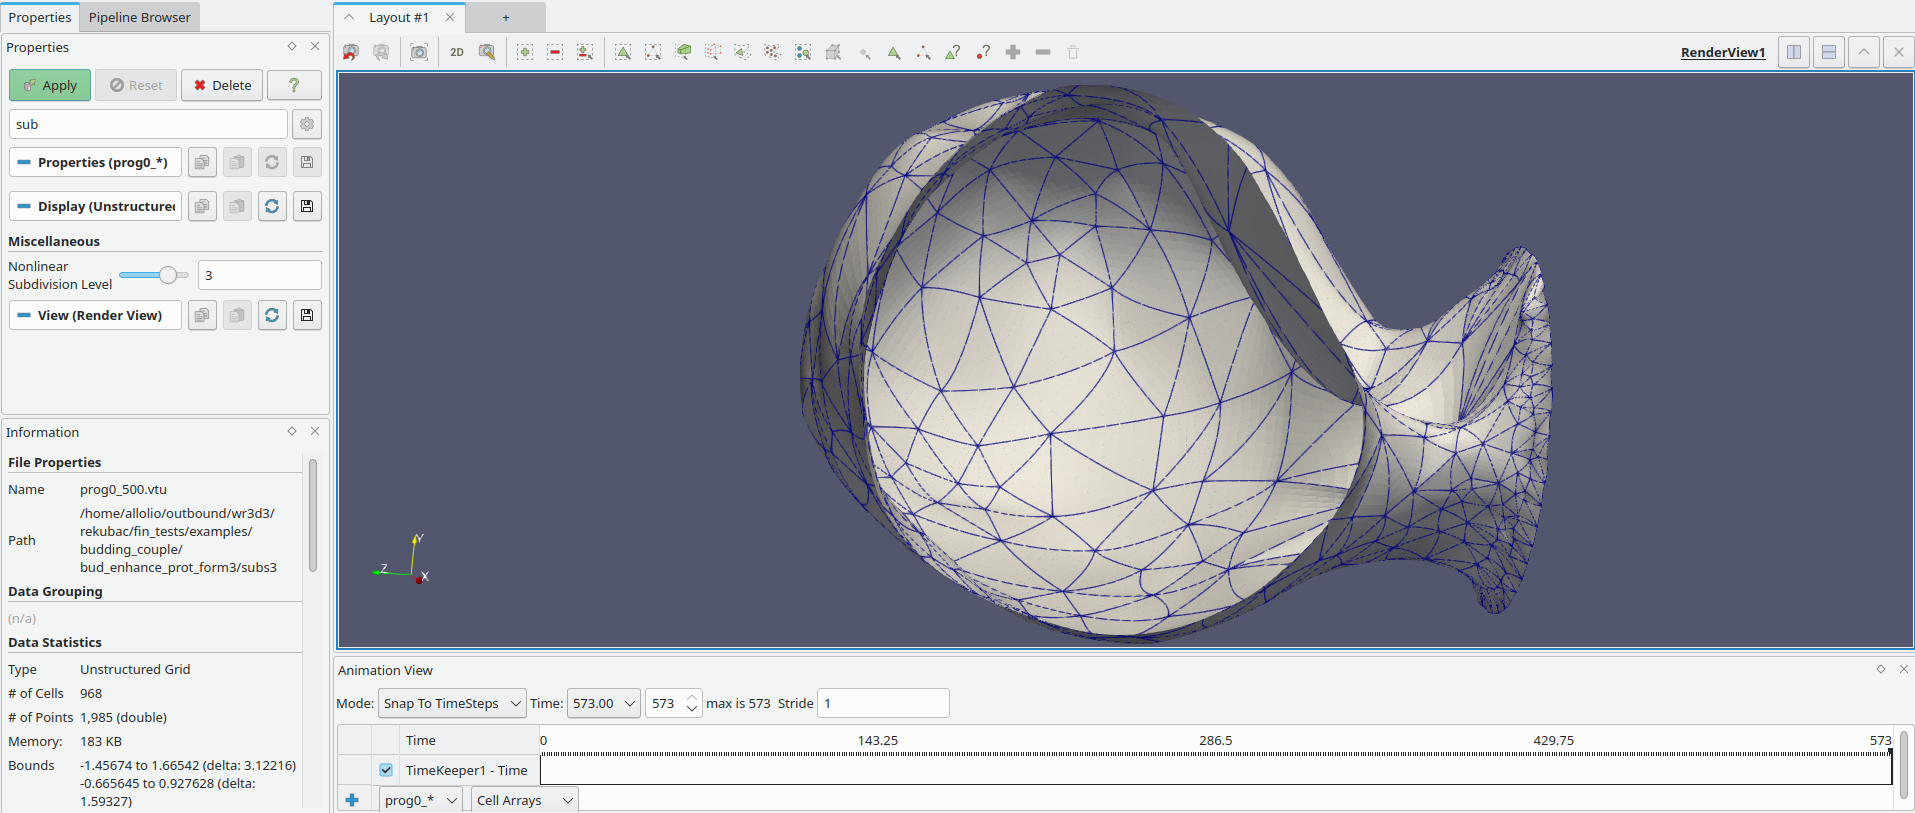
\includegraphics[width=\linewidth]{subdivision.png}
    \caption{Paraview allows the visualization of curved elements. While these are not exactly identical to the Nagata elements, they are close enough}
    \label{fig:curved}
\end{figure}

\begin{figure}[h]
    \centering
    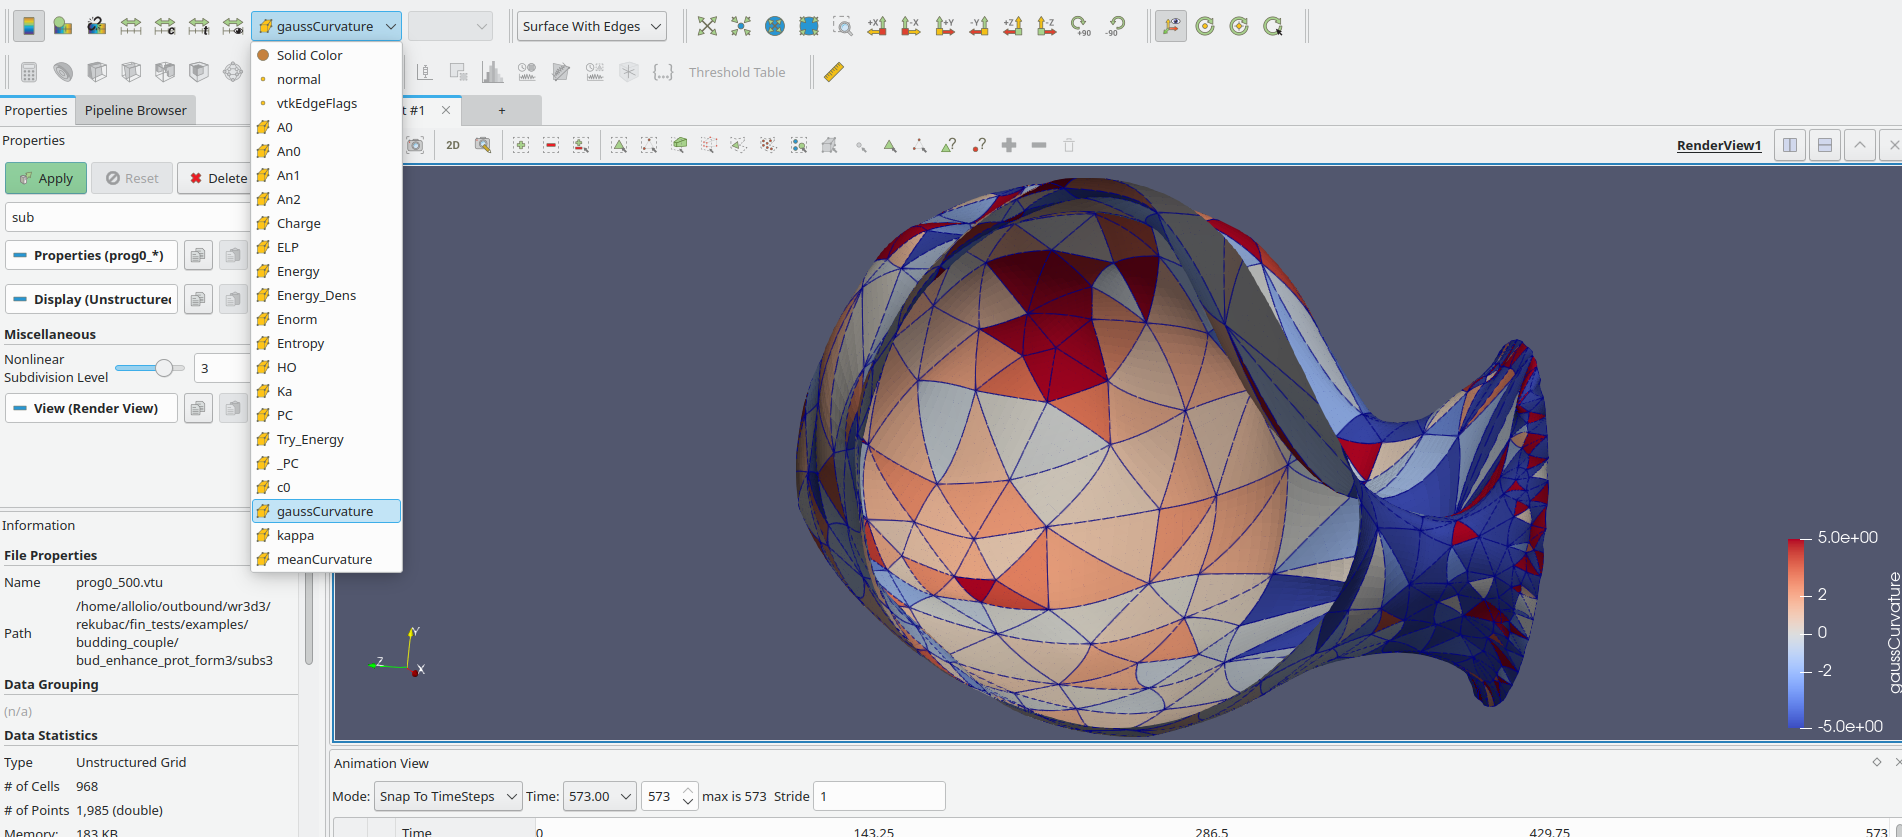
\includegraphics[width=\linewidth]{choice.png}
    \caption{Paraview provides access to many quantities amenable to visualization. Lipid types are automaticall exported into the vtu files.}
    \label{fig:choice}
\end{figure}

The \textsc{OBJ} files created by the program can also be visualized in paraview, but are compatible with rendering sofwarew, such as \textsc{blender}. A \textsc{gnuplot} compatible file, $out.plt$ is created at the end of a simulation. It can be plotted e.g. by calling

\begin{verbatim}
    splot "out.plt" using 1:2:3 w l
\end{verbatim}
inside \textsc{gnuplot}. For more information see the respective software documentations of these tools.

% \section{Advanced Usage}


\section{Tips on Simulation Planning and Execution}

\subsection{Basic Strategy}
\begin{enumerate}
    \item Each run should be done in its own subdirectory, to avoid overwriting files. Make sure all input files are present.
\item At the beginning of the simulation parameters should be fine tuned. This means, that instead of going directly into production very small runs of 10-500 steps, with low reporting intervals should be performed.
\item The console output should be studied for warnings, it should be checked, if blocks are correctly read in. 
\item the \textbf{scale} of the mesh should be examined. Find the mesh scale
\begin{verbatim}
    INFO: Average Edge Length
\end{verbatim}
as well as the initial volume, area and energy in the output. Your neighbourlist cutoff should be larger than the average edge lenght at least. 
\item Run with good behavior by setting restraint targets to or close to the intial values.
\item It makes sense to compare DCH and CHF energies to check if A$_0$ values are reasonable.
\item It can make sense to run with very low $\kappa$ or $\beta$ for short time, so see the direction things take.
\item Check the 
\begin{verbatim}
    G1 Diagnostic
\end{verbatim}
value it should remain above 0.94.
\end{enumerate}
\noindent
\textbf{In particular check/plot columns of the report file to see if quantitites explode or behave in an anomalous manner. Read the follow on sections on setting K$_A$ A$_0$ LAMBDAS and DEFS}

\subsection{How to set targets and penalties}

When setting DEF and LAMBDA values for your simulation, the LAMBDA has to be high enough to ensure the corresponding property is tightly controlled. One example would be that e.g. 5 \% deviation from the targed would be about 10 \% of the total energy of the system. The report file and initial dry runs can be used to estimate this total energy.
Consequently your DEF target value is very far from the current state, you risk wrecking the mesh by dominating all other energy (including penalty) terms. Either set LAMBDA it so low, that even initially the penalty is only some tens of percents of the intial energy or use the INCR mechanism to gradually get to the target. It is possible to combine these techniques. The individual surface penalties $K_A$ should also be chosen in a scale-depdendent manner. A tenfold increase in triangle surface should cost more than the average energy per triangle etc.

\subsection{How to optimize performance}

If at all possible, use a high quality equilateral mesh. Remeshing can be done, e.g. using meshlab.
My rules of thumb for optimizing performances is,
\begin{itemize}
    \item Keep the neighbor list cutoff as small as possible. If necessary trade frequent neighbor list updates for short cutoffs. It is possible to use restarts to continue before an overlap occurs.
    \item Monte Carlo step size above acceptance rate. It is recommended to set e.g. the initial step size of the Vertex step to ca. 2-3 x the average edge length, then set autoadjust for 200-1000 steps and then increase the final result by ca. 20 \%
    This applies only to vertex steps, normal steps should be kept around 1.
    \item Keep the mesh as small as possible. It should not be necessary to use much more than 1000 faces for any cell shape. If necessary use blocks and cutouts to restrict the size.
    \item Use a workstation with many cores and good single core performance.
\end{itemize}

\subsection{How to monitor accuracy}

The worst problems arise either from mesh degeneration or from too high MC steps. If a phenomenon looks surprising, there are two main ways to get better results
\begin{enumerate}
    \item reducing the step size or 
    \item controlling the mesh with A$_0$ and K$_A$ values.
\end{enumerate}
If the G1 criterion in the report falls below 0.85, the simulation is very likely producing complete garbage, at least at that moment. 
The energy contributions should be decomposed, too high penalties indicate wrong DEFs, too high energies, can be due to too high MC steps or wrong parameters. 
Monitor the mesh with paraview, and look at the homogeneity of areas, triangle sizes should not be different by several orders of magnitude.
Triangles can be controlled on an individual level using K$_A$.
Long-term drifts against a penalty are a sign of the breakdown of reversibility and must be tackled. Please check the various energy functional descriptions for further advice, specific to a situation.

\subsection{How to set boundary conditions}

The way to set geometric boundary conditions is via the blocks.txt file. For example, it is possible to set a Dirichlet boundary conditions of the membrane, i.e. fixed coordinates by fixing the vertices at the boundary in the blocks.txt file, using, e.g. the tool described in this section. If the normals on the boundary are also frozen then so is the entire edge interpolant and hence also a tangent vector along the edge. 
Going further inward allows to ensure a good measure of tangen continuity on the edges. More sophisticated partial blockades are also possible using components of the vectors, e.g. restraining the boundary to a plane. By setting Edge blocks, it is e.g. possible to set a region of fixed lipid composition. Any combination of blockades is possible. See Section 5.6 and the examples for more details.

\bibliography{ref}
\end{document}
